\section{Stable Diffusion}
\label{sec:stable_diffusion}

\begin{figure}
    \centering
    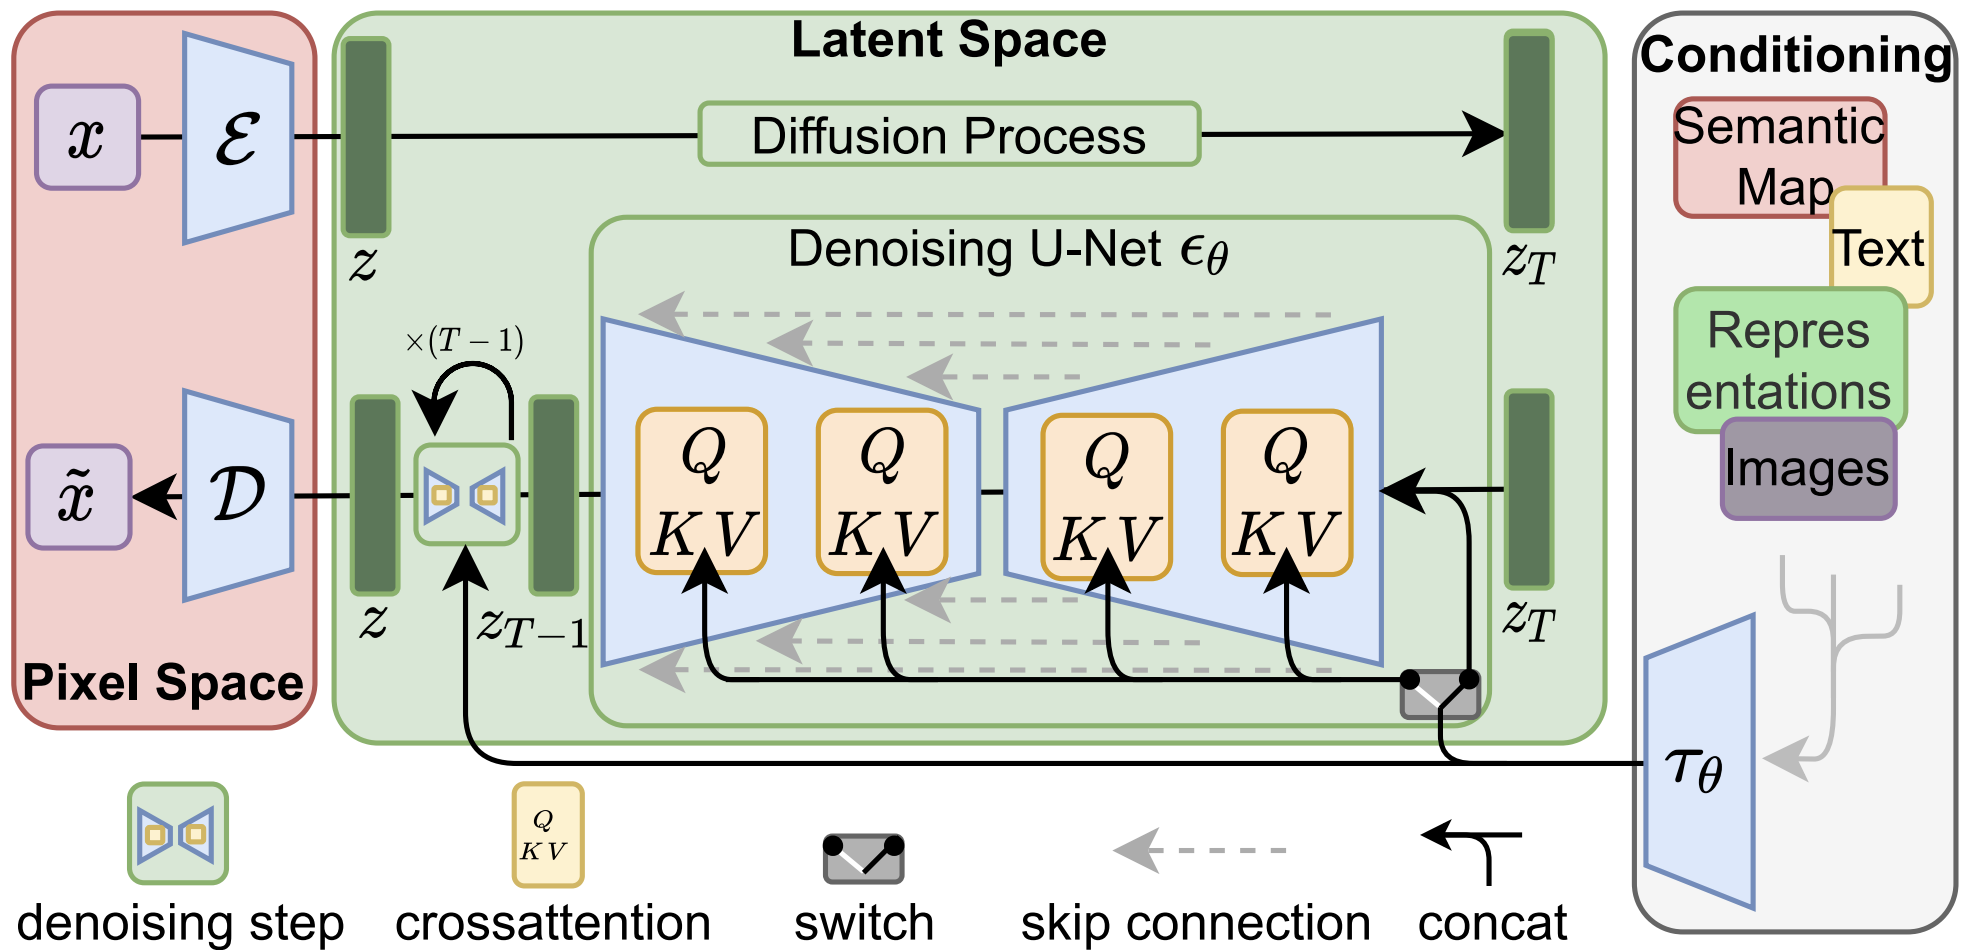
\includegraphics[width=1\textwidth]{images/diffusion_models/stable_diffusion.png}
    \caption{Stable diffusion process in Stable Diffusion Models (SDMs) \cite{stable_diffusion}.}
    \label{fig:stable_diffusion}
\end{figure}

Stable diffusion models are based on latent diffusion. In the paper \cite{stable_diffusion} the authors suggested that computing gradients directly on RGB space is inefficient, since this space is high-dimentional. Instead, they suggest to first convert the training images to a lower-dimensional latent space and then apply the diffusion processes on this space.

This process is much more efficient, and in the paper \cite{stable_diffusion} the authors showed that the model can be trained on a single GPU with 16GB of memory. The model is trained on a 256x256 resolution CelebA-HQ dataset with 30 diffusion steps.

An example of this is when giving an image to a person and asking them to describe the image, they will not describe the individual pixel values, but instead describe the high-level features of the image first.

A 2021 paper released by OpenAI \cite{openai_diffusion_beats_gans} shows that diffusion models can outperform GANs in terms of image fidelity by trading off diversity.